\documentclass[abstract=on,10pt,a4paper,bibliography=totocnumbered]{article}
\usepackage[paper=a4paper,left=35mm,right=35mm,top=25mm,bottom=30mm]{geometry}
\usepackage[doublespacing]{setspace}
\usepackage[english]{babel}
\usepackage[utf8]{inputenc}
\usepackage[round]{natbib}
\usepackage{amsmath}
\usepackage{colortbl}
\usepackage{amsfonts}
\usepackage{amssymb}
\usepackage{gensymb}
\usepackage{graphicx}
\usepackage{tikz}
\usepackage{enumerate}
\usepackage{enumitem}
\usepackage{subcaption}
\usepackage{booktabs}
\usepackage[hidelinks]{hyperref}
\usepackage[nameinlink]{cleveref}
% \usepackage{lineno}
\usepackage{multirow}
\usepackage{arydshln}
\usepackage[flushleft]{threeparttable}
\usepackage[nomarkers, nolists]{endfloat}
\usepackage[colorinlistoftodos]{todonotes}

%------------------------------------------------------------------------------
%	Some Styling
%------------------------------------------------------------------------------
% Creating some TikZ styles
\tikzset{
  nonterminal/.style = {rectangle
    , minimum size = 6mm
    , very thick
    , draw = black!
  }
}

% Changing the style of captions in figures etc.
\captionsetup{labelfont=bf, format=plain, font=small}

% Change how equations are referenced
\renewcommand{\theequation}{Equation \arabic{equation}}%

%------------------------------------------------------------------------------
%	Titlepage: Header
%------------------------------------------------------------------------------
\title{Step by Step: Using Step Selection Functions to Simulate Dispersal and
Assess Landscape Connectivity}

% \title{Step by Step: The Utility of Dispersal Simulations to Assess Landscape
% Connectivity}

% List of Authors
\author{
  David D. Hofmann\textsuperscript{1,2,\S} \and
  Gabriele Cozzi\textsuperscript{1,2} \and
  John W. McNutt\textsuperscript{2} \and
  Arpat Ozgul\textsuperscript{1} \and
  Dominik M. Behr\textsuperscript{1,2}
}

% Reduce spacing between authors
\makeatletter
\def\and{%
  \end{tabular}%
  \hskip -0.5em \@plus.17fil\relax
  \begin{tabular}[t]{c}}
\makeatother

% Current Date
\date{\today}

% And here the masterpiece begins
\begin{document}

% Change page numbering
\pagenumbering{gobble}

% Required to be able to cite
\bibliographystyle{apalike}

% Create Titlepage
\maketitle

%------------------------------------------------------------------------------
%	Titlepage: Additional Info
%------------------------------------------------------------------------------
\begin{flushleft}

\vspace{0.5cm}

\textsuperscript{1} Department of Evolutionary Biology and Environmental
Studies, University of Zurich, Winterthurerstarsse 190, 8057 Zurich,
Switzerland.

\textsuperscript{2} Botswana Predator Conservation, Private Bag 13, Maun,
Botswana.

\textsuperscript{\S} Corresponding author (david.hofmann2@uzh.ch)

\vspace{4cm}

\textbf{Running Title:} Release the Dogs! Simulating Wild Dog Dispersal to
Assess Landscape Connectivity

\vspace{0.5cm}

\textbf{Keywords:} dispersal, simulation, movement, integrated step selection
function, Kavango-Zambezi Transfrontier Conservation Area, landscape
connectivity, Lycaon pictus

\end{flushleft}

%------------------------------------------------------------------------------
%	Abstract
%------------------------------------------------------------------------------
\newpage
\begin{abstract}
%------------------------------------------------------------------------------
% Short Version
%------------------------------------------------------------------------------
\textbf{Short Version }
The ability to disperse is contingent on a sufficient degree of landscape
connectivity, which is why the identification and preservation of movement
corridors that promote connectivity has become a task of extraordinary
importance. Currently, ecologists rely on least-cost analysis or circuit
theory to investigate connectivity, albeit both methods make several
assumptions that are hardly met in reality. To address these issues,
simulations from individual-based movement models have been proposed, yet a
unified framework to simulate dispersal and quantify connectivity is lacking.

Here, we propose a simple three-step workflow that combines several
already-existing methods to assess connectivity using simulated dispersal
trajectories. In step one, we use integrated step selection functions to
parametrize a mechanistic movement model rendering dispersal behavior. In step
two, we apply the parametrized model as an individual-based movement model to
simulate dispersal trajectories. In step three, we combine simulated
trajectories into three complementary connectivity maps, each focusing on a
different aspect of landscape connectivity.

We showcase the application of the proposed workflow using data of dispersing
African wild dogs (\textit{Lycaon pictus}) and assess landscape connectivity
within the world's largest transboundary conservation area in Southern Africa.
We thereby shed light into dispersing wild dogs' habitat and movement
preferences, while also uncovering crucial dispersal corridors. With this
analysis, we demonstrate that simulations from integrated step selection
functions offer a simple, yet powerful alternative to traditional connectivity
modeling techniques.
\end{abstract}

\newpage
\begin{abstract}
%------------------------------------------------------------------------------
%  LONG VERSION
%------------------------------------------------------------------------------
\textbf{Long Version }
Dispersal of individuals is crucial for long-term species persistence and
depends on a sufficient degree of landscape connectivity. To date, researchers
primarily investigate connectivity using least-cost analysis and circuit theory,
both methods that make assumptions which are hardly met in reality. Least-cost
analysis assumes that animals move towards a known endpoint and are
knowledgeable about the most favorable route to reach it. Circuit theory
presumes a complete random walk and therefore fails to incorporate directional
persistence. These shortcomings can be overcome by spatio-temporally explicitly
simulating dispersal, yet a unified approach for such simulations is lacking.

Here, we present a simple three-step workflow to simulate dispersal and assess
connectivity starting from empirical GPS movement data. In step one, we use
integrated step selection functions to fit a mechanistic movement model
describing habitat and movement preferences of dispersers. In step two, we apply
the parameterized model to simulate individual dispersal trajectories. In step
three, we combine the simulated trajectories into three complementary
connectivity maps: a heatmap that highlights frequently traversed areas, a
betweenness map that pinpoints dispersal corridors, and a map of inter-patch
connectivity that indicates the presence and intensity of functional links
between habitat patches. As a case study, we analyse data on the endangered
African wild dog and assess landscape connectivity in the Kavango-Zambezi
Transfrontier Conservation Area, the world’s largest transboundary conservation
area.

Our results show that wild dogs preferably disperse with directional persistence
in the vicinity to water bodies and through areas with little human influence and
sparse woodland cover. Dispersal simulations and subsequent connectivity maps
revealed several dispersal hotspots and corridors across the extent of the
KAZA-TFCA. Connectivity between NPs inside the KAZA-TFCA was good, yet few
dispersers successfully moved from Zambia's NPs into neighboring areas.

We show that simulations from step-selection functions offer a simple yet
powerful alternative to traditional connectivity modeling techniques. In
contrast to traditional connect modeling techniques, simulations not only make
fewer unrealistic assumptions but also permit a more mechanistic understanding
of dispersal and landscape connectivity. This makes our workflow useful for a
variety of applications in ecological, evolutionary, and conservation research.

\end{abstract}

%------------------------------------------------------------------------------
%	Main Text
%------------------------------------------------------------------------------
\newpage

\onehalfspacing
\tableofcontents
\doublespacing

% Change page numbering
\newpage
\pagenumbering{arabic}

% Create linenumbers
% \linenumbers

\section{Introduction}

% Importance of Dispersal & Connectivity
\subsection{Importance of Connectivity \& Connectivity Models}
Dispersal of individuals is a vital process that allows species to maintain
genetic diversity \citep{Perrin.1999, Perrin.2000, Frankham.2002, Leigh.2012,
Baguette.2013}, rescue non-viable populations \citep{Brown.1977}, and colonize
unoccupied habitats \citep{Hanski.1999b, MacArthur.2001}. Importantly, the
ability to disperse depends on a sufficient degree of landscape connectivity
\citep{Fahrig.2003, Clobert.2012}, making the identification and protection of
dispersal corridors that promote connectivity a task of fundamental importance
\citep{Nathan.2008, Doerr.2011, Rudnick.2012}. The identification of dispersal
corridors not only necessitates a comprehensive understanding of the factors
that limit dispersal, but also an appropriate model to estimate connectivity
\citep{Baguette.2013, Vasudev.2015, Hofmann.2021}. To date, the two most
commonly used connectivity models are least-cost path analysis (LCPA;
\citealp{Adriaensen.2003}) and circuit theory (CT; \citealp{McRae.2006,
McRae.2008}), both graph-based methods that quantify conductance of the
landscape based on habitat permeability \citep{Zeller.2012}. However, both
approaches rest on assumptions that appear unsuitable for dispersers, which is
why simulating dispersal from individual-based movement models provides a
promising alternative approach to investigate connectivity \citep{Diniz.2019}.

% Issues with Both Methods
\subsection{Issues with Traditional Connectivity Models}
Traditional connectivity models make assumptions that are rarely met for
dispersers. LCPA, for instance, assumes that individuals move towards a
preconceived endpoint and choose a cost-minimizing route accordingly
\citep{Sawyer.2011, Abrahms.2017}. While this assumption may be fulfilled by
migrating animals, it is unlikely to hold for dispersers, as dispersers
typically move across unfamiliar territory, so the associated movement costs and
potential endpoints are unknown to them \citep{Koen.2014, Cozzi.2020}. CT, on
the contrary, posits that animals move according to a random walk, entailing
that autocorrelation between subsequent movements cannot be rendered
\citep{Diniz.2019}. For dispersers, however, autocorrelated movements are
regularly observed \citep{Cozzi.2020, Hofmann.2021}, implying that dispersal
trajectories are usually strongly directional. Moreover, graph-based methods are
unable to reflect the temporal dimension of dispersal, so that statements about
the expected duration for moving between habitats are impossible
\citep{Martensen.2017, Diniz.2019}.

% What about IBMMs?
\subsection{What about IBMMs?}
The shortcomings inherent to LCPA and CT can be overcome by simulating dispersal
from individual-based movement models (IBMMs) and converting simulated
trajectories into meaningful measures of connectivity \citep{Diniz.2019}). In
contrast to graph-based methods, IBMMs allow to explicitly simulate how
individuals move across and interact with the encountered landscape
\citep{Kanagaraj.2013, Clark.2015, Allen.2016, Hauenstein.2019, Zeller.2020}, as
well as to render potential interactions between movement behavior and habitat
conditions, thus shifting the focus from a structural to a more functional view
on connectivity \citep{Tischendorf.2000, Kanagaraj.2013, Hauenstein.2019}.
Furthermore, because simulations from IBMMs generate movement sequentially, the
temporal dimension of dispersal becomes explicit and allows to model
autocorrelation between subsequent movements \citep{Diniz.2019}. Finally,
simulations from IBMMs do not enforce connections towards preconceived
endpoints, thereby mitigating biases arising from misplaced endpoints. Despite
these advantages, a unified framework to simulate dispersal and assess
connectivity using IBMMs is lacking.

% Proposed Solution: Three-Step Workflow
\subsection{Proposed Solution: Three-Step Workflow}
Here, we draw on recent advancements in movement ecology and propose a simple
three-step workflow for simulating dispersal and assessing landscape
connectivity (\Cref{GraphicalAbstract}). In step one, we combine GPS movement
data of dispersing individuals with relevant habitat covariates to fit a
mechanistic movement model using integrated step selection functions (ISSFs,
\citealp{Avgar.2016}). ISSFs permit inference on the focal species' habitat
kernel (i.e. habitat preferences), its movement kernel (i.e. movement
preferences/capabilities), and potential interactions between the two
\citep{Avgar.2016, Fieberg.2021}. In step two, we simulate individual dispersal
trajectories using the parametrized movement from step one. Comparable
simulations have already been employed to estimate steady-state utilization
distributions of residents \citep{Potts.2013, Signer.2017} and to model
landscape connectivity, yet disregarding interdependencies between habitat and
movement kernels \citep{Clark.2015, Zeller.2020}. Finally, in step three, we
convert simulated trajectories into three complementary connectivity maps, each
highlighting a different aspect of connectivity. The set of maps includes (i) a
heatmap revealing areas that are frequently traversed by simulated dispersers
(e.g. \citealp{Hauenstein.2019, Zeller.2020}), (ii) a betweenness-map
delineating dispersal corridors and bottlenecks (e.g.
\citealp{BastilleRousseau.2018}), (iii) and a map of inter-patch connectivity,
depicting the presence and intensity of use of specific connections, as well as
the average dispersal duration required to connect corresponding habitat patches
(e.g. \citealp{Gustafson.1996, Kanagaraj.2013}).

% Introduction of the study species
\subsection{Case Study}
We showcase the application of the proposed workflow (\Cref{GraphicalAbstract})
using dispersal data collected on the endangered African wild dog
(\textit{Lycaon Pictus}). The African wild dog represents a highly mobile
species whose persistence hinges on a sufficient degree of landscape
connectivity. Once common throughout sub-Saharan Africa, this species has
disappeared from much of its historic range, largely due to human persecution,
habitat fragmentation, and disease outbreaks \citep{Woodroffe.2012}. Wild dogs
typically disperse in single-sex coalitions \citep{McNutt.1996, Behr.2020} and
are capable of dispersing several hundred kilometers \citep{DaviesMostert.2012,
Masenga.2016, Cozzi.2020}. Although previous studies have investigated
connectivity using LCPA \citep{Hofmann.2021} or CT \citep{Brennan.2020}, a more
comprehensive and mechanistic understanding of connectivity is missing for this
species (but see \citealp{Creel.2020}). With fewer than 6,000 free-ranging wild
dogs remaining in fragmented populations \citep{Woodroffe.2012}, reliable
information on landscape connectivity is essential for the conservation of this
endangered carnivore. Here, we use GPS data of 16 dispersing wild dogs
originating from a free-ranging population in northern Botswana to parametrize a
mechanistic movement model, which we then employed to simulate 80,000 dispersal
trajectories across the landscape of the world's largest transboundary
conservation area, the Kavango-Zambezi Transfrontier Conservation Area
(KAZA-TFCA). We anticipated that simulations based on our three-step workflow
would overcome several of the above highlighted conceptual shortcomings of
traditional connectivity models and provide a more comprehensive view of
landscape connectivity

\begin{figure}[htbp]
  \begin{center}
    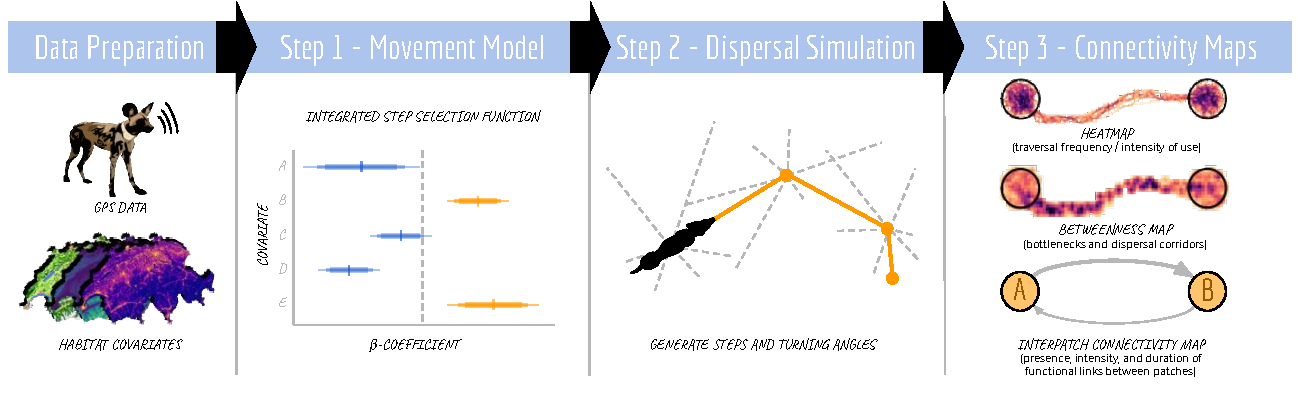
\includegraphics[width = \textwidth]{99_GraphicalAbstract2.pdf}
    \caption{Flowchart of the simulation-based connectivity analysis as proposed
    in this article. First, GPS data and habitat covariates must be
    collected. The combined data is then analyzed in an integrated step
    selection model, which enables the parametrization of the focal species'
    habitat and movement kernels and results in a mechanistic movement model.
    The parametrized model is then treated as an individual-based movement model
    and used to simulate dispersal trajectories. Ultimately, simulated
    trajectories serve to produce a set of maps that are pertinent to landscape
    connectivity. This includes a heatmap, indicating the traversal frequency
    across each spatial unit of the study area, a betweenness map, highlighting
    movement corridors and bottlenecks, and, finally, an inter-patch
    connectivity map, where the frequency of connections and their average
    duration can be depicted.}
    \label{GraphicalAbstract}
  \end{center}
\end{figure}

\section{Methods}
\subsection{Study Area}
The study area centered at -17\degree 13'9''S, 23\degree 56'4''E
(\Cref{StudyArea}a) was located in southern Africa (\Cref{StudyArea}a) and
spanned more than 1.3 Mio. km\textsuperscript{2}, encompassing the entire
KAZA-TFCA (\Cref{StudyArea}b). The KAZA-TFCA comprises parts of Angola,
Botswana, Namibia, Zimbabwe, and Zambia and hosts a rich diversity of
landscapes, ranging from savannah to grassland and from dry to moist woodland
habitats. In its center lies the Okavango Delta, a dominant hydro-geographical
feature and the world's largest flood-pulsing inland delta. Large portions of
the KAZA-TFCA are part of designated national parks (NPs) and other protected
areas, yet considerable human influence through roads, agricultural sites, and
settlements remains.

\begin{figure}[h]
  \begin{center}
    \begin{tikzpicture}
        \node[anchor=south west,inner sep=0] (image) at (0,0,0) {
        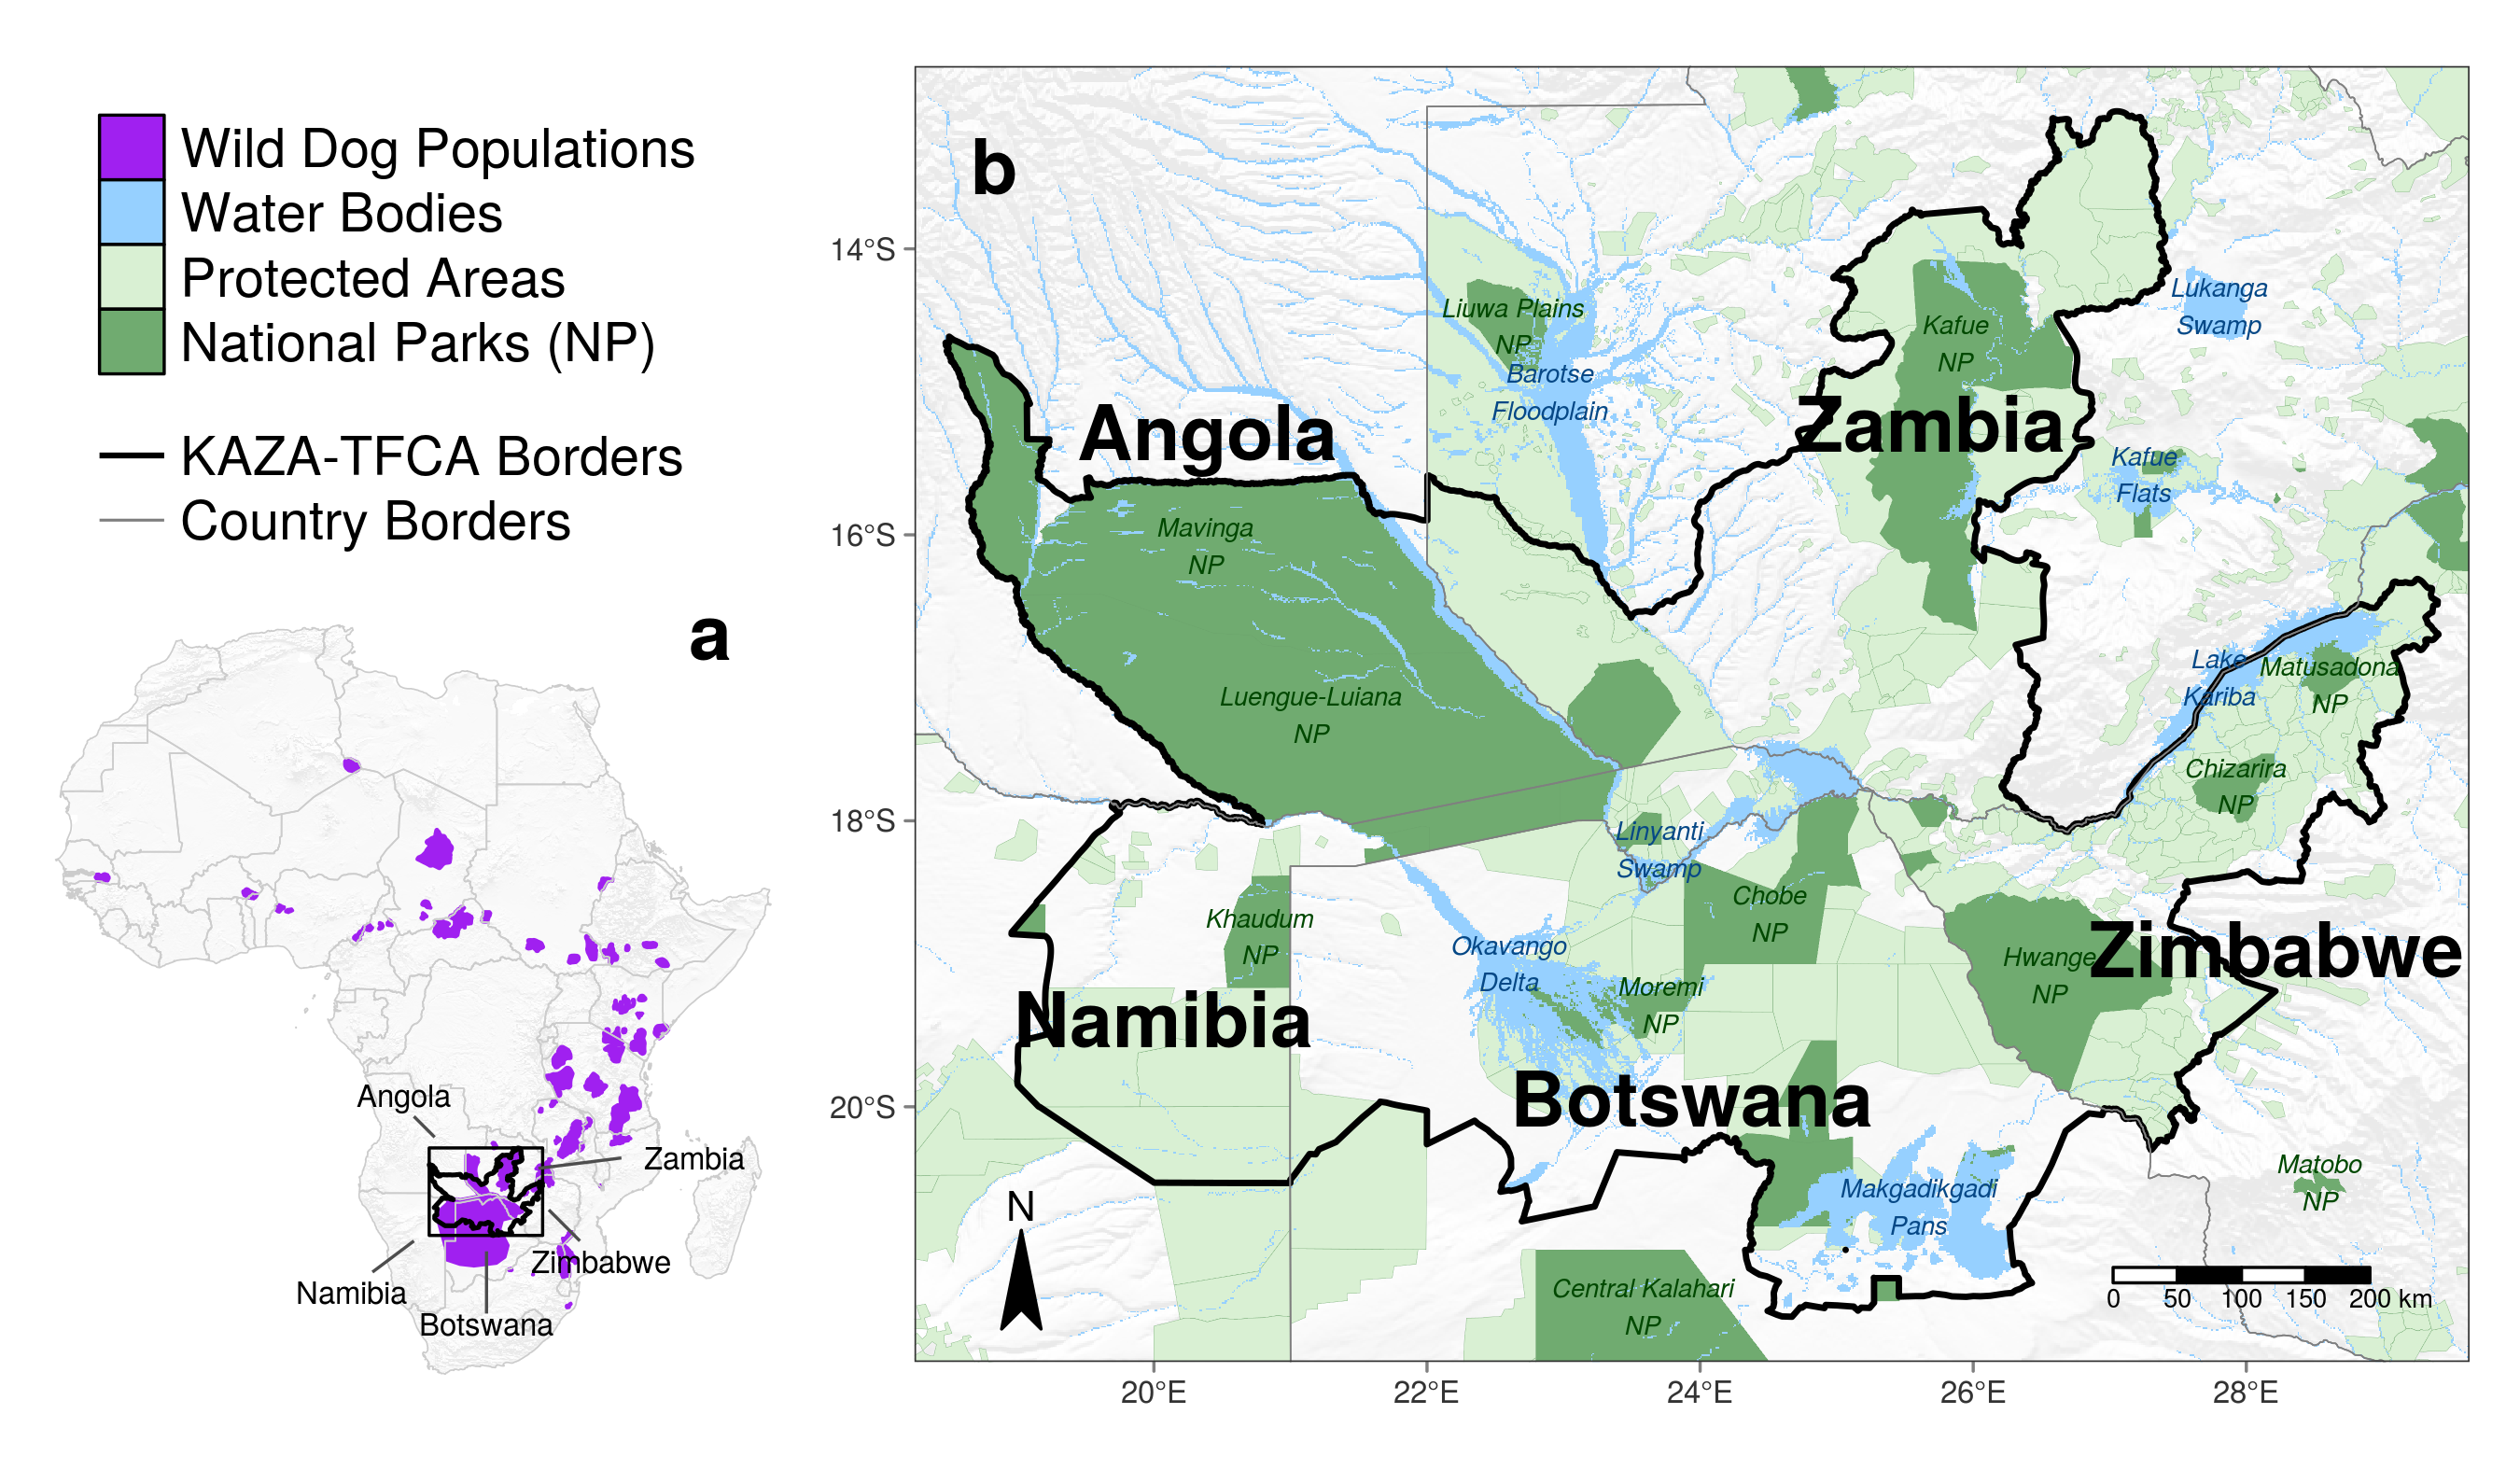
\includegraphics[width=\textwidth]{99_StudyArea.png}
        };
        \begin{scope}[x={(image.south east)},y={(image.north west)}]
            % % next four lines will help you to locate the point needed by forming a grid.
            % % comment these four lines in the final picture.
            % \draw[help lines,xstep=.1,ystep=.1] (0,0) grid (1,1);
            % \draw[help lines,xstep=.05,ystep=.05] (0,0) grid (1,1);
            % \foreach \x in {0,1,...,9} { \node [anchor=north] at (\x/10,0) {0.\x}; }
            % \foreach \y in {0,1,...,9} { \node [anchor=east] at (0,\y/10) {0.\y};}
            % % upto here
            \draw[densely dotted, blue] (0.169, 0.222) -- (0.364, 0.955);
            \draw[densely dotted, blue] (0.169, 0.157) -- (0.364, 0.074);
        \end{scope}
    \end{tikzpicture}
    \caption{Illustration of the study area located in southern Africa. (a) The
    study area was confined by a bounding box spanning the entire KAZA-TFCA
    which comprises parts of Angola, Namibia, Botswana, Zimbabwe, and Zambia.
    (b) The KAZA-TFCA currently represents the world's largest terrestrial
    transfrontier conservation area, covering a total area of 520'000
    km\textsuperscript{2}. Its main purpose is to re-establish connectivity
    between already-existing NPs (dark green) and other protected areas (light
    green).}
    \label{StudyArea}
  \end{center}
\end{figure}

\subsection{Data Collection and Preparation}
\subsubsection{GPS Data}
We collected GPS movement data on 16 dispersing wild dogs (7 females and 9
males) between 2011 and 2019 from a free-ranging population in northern Botswana
(details on the data collection can be found in \cite{Cozzi.2020} and
\cite{Hofmann.2021}). Because behavior during dispersal is more pertinent to
landscape connectivity than behavior during residence \citep{Elliot.2014,
Abrahms.2017}, we discarded data collected when individuals were resident. We
determined the exact timing of emigration and settlement using direct field
observations and through visual inspection of the net squared displacement (NSD)
metric. NSD measures the squared Euclidean distance of a GPS relocation to a
reference point \citep{Borger.2012}, which we set to the center of each
dispersers' natal home range. Thus, dispersal was deemed to have started once an
individual left its natal home range and ended once the NSD metric remained
constant, indicating settlement. During dispersal, GPS collars recorded a fix
every 4 hours and regularly transmitted data over the Iridium satellite system.
To ensure regular timespans between GPS fixes, we removed any fix that was not
successfully obtained on the aspired 4-hourly schedule (allowing for a tolerance
of \( \pm \) 15 minutes). We then converted the remaining fixes (n = 4'169) into
steps, where each step represented the straight-line movement between two
consecutive GPS fixes \citep{Turchin.1998}.

\subsubsection{Habitat Covariates}
We represented the physical landscape in our study area by the habitat
covariates \textit{water-cover, distance-to-water, woodland-cover,
shrub/grassland-cover, and human-influence}. To correctly render seasonality in
water-cover, we applied a remote sensing algorithm that enabled us to obtain
weekly updated raster-layers for water-cover and corresponding layers for
distance-to-water from MODIS satellite imagery \citealp{Wolski.2017,
Hofmann.2021}. This algorithm is now implemented in the \textsf{floodmapr}
package which is available on GitHub
(\url{https://github.com/DavidDHofmann/floodmapr}). Using the frequently updated
floodmpas we were able to correctly assign the most appropriate covariate layer
to each observed movement step. To ensure a consistent resolution across habitat
covariates, we coarsened or interpolated all layers to a resolution of 250 m x
250 m. A detailed description of how we prepared each habitat covariate is
provided in \cite{Hofmann.2021}.

Besides habitat covariates, we computed movement metrics that we used as
movement covariates in ISSF models \citep{Avgar.2016, Fieberg.2021}. Movement
metrics were calculated for each step and included the step length
(\textsf{sl}), its natural logarithm (\textsf{log(sl)}), and the cosine of the
relative turning angle (\textsf{cos(ta)}). Moreover, we created the binary
variable \textsf{LowActivity} indicating whether a step was realized during
periods of low wild dog activity (09:00 to 17:00 local time) or high wild dog
activity (17:00 to 09:00 local time, \citealp{Cozzi.2012}). We performed all
data preparations, spatial computations, and statistical analysis in R, version
3.6.6 \citep{R.2020}. Some helper functions were written in {\tt C++} and
imported into {\tt R} using the {\tt Rcpp} package \citep{Eddelbuettel.2011,
Eddelbuettel.2013}.

\subsection{Step 1 - Movement Model}
We used ISSFs to parametrize a mechanistic movement model for dispersing wild
dogs \citep{Avgar.2016}. More specifically, we paired each realized step with 24
random steps, so that a realized step plus its 24 random steps formed a
25-step-stratum that received a unique identifier. As suggested by
\cite{Avgar.2016}, we generated random steps by sampling random turning angles
from a uniform distribution (\(-\pi, +\pi\)) (which is equivalent to a von Mises
distribution with location and concentration parameters; \(\mu = \kappa = 0\))
and step lengths from a gamma distribution that was fitted to realized steps
(scale \(\theta\) = 6'308 and shape \(k\) = 0.37). Along each step, we extracted
and averaged values from the habitat covariate layers using the {\tt velox}
package \citep{Hunziker.2021} and calculated the movement metrics \textsf{sl},
\textsf{log(sl)}, and \textsf{cos(ta)} for each realized and random step. To
facilitate model convergence, we standardized all continuous covariates to a
mean of zero and a standard deviation of one. Since correlation among covariates
was low (\(|r| < 0.6\); \citealp{Latham.2011}), we retained all of them for
modeling.

To contrast realized steps (scored 1) and random steps (scored 0), we assumed
that animals assigned a selection score \(w(x)\) of the exponential form to each
step (\ref{EQ2}; \citealp{Fortin.2005}). \(w(x)\) depended on the step's
associated covariates (\(x_1, x_2, ..., x_n\)) and on the animal's preferences
(i.e. relative selection strengths; \citealp{Avgar.2017}) towards these
covariates (\(\beta_1, \beta_2, ..., \beta_n\)):

\begin{equation}
\label{EQ1}
  w(x) = exp(\beta_1 x_1 + \beta_2 x_2 + ... + \beta_n x_n)
\end{equation}

\noindent The probability of a step being realized was then contingent on the
step's selection score, as well as on the selection scores of all other step in
the same stratum:

\begin{equation}
\label{EQ2}
  P(Y_{i} = 1 | Y_{1} + Y_{2} + ... + Y_{i} = 1) =
  \frac{w(x_{i})}{w(x_{1}) + w(x_{2}) + ... + w(x_{i})}
\end{equation}

\noindent To estimate preferences (i.e. the \(\beta\)-coefficients), we used
mixed effects conditional logistic regression analysis \citep{Muff.2020} that we
implemented using the r-package {\tt glmmTMB} \citep{Brooks.2017}. To capitalize
on the poisson trick proposed by \cite{Muff.2020}, we defined random intercepts
for each stratum and fixed the intercept variance to an arbitrary high value of
\(10 ^ 6\). We also used disperser identity to model random slopes for all
covariates.

The covariate structure of the movement model was based on a habitat selection
model that we previously developed for dispersing wild dogs (hereafter referred
to as \textit{based model}, \citealp{Hofmann.2021}). In the base model, no
interactions among habitat covariates and movement covariates were considered.
Hence, we expanded the base model and allowed for interactions between all
movement covariates and habitat covariates, thus reflecting that movement
behavior may depend on habitat conditions (details in Appendix A1). To determine
the most parsimonious movement model among model candidates, we ran stepwise
forward model selection based on Akaike's Information Criterion (AIC,
\citealp{Burnham.2002}). Finally, we validated the predictive power of the most
parsimonious model using k-fold cross-validation for case-control studies as
described in \cite{Fortin.2009}. This validation proofs a significant prediction
in case the Spearman rank correlation of predicted step-ranks and associated
frequencies under the movement model is significantly greater than under the
assumption of random preferences (details in Appendix A2).

\subsection{Step 2 - Dispersal Simulation}
We used the most parsimonious movement model to simulate individual dispersal
trajectories within the study area. The simulation of a dispersal trajectory
resembled an ``inverted'' ISSF and was set up as follows. (1) We defined a
random source point and assumed a random initial orientation of the animal. (2)
Starting from the source point, we generated 25 random steps by sampling turning
angles from a uniform distribution (\(-\pi, +\pi\)) and step lengths from our
fitted gamma distribution. Like in the empirical data, each random step
represented the straight-line movement possible within 4 hours. To prevent
unreasonably large steps, we restricted sampled step lengths to a maximum of 35
km (i.e. the farthest dispersal distance traveled within 4 hours in our data).
(3) Along each random step, we extracted and averaged values from the different
habitat covariate layers and calculated movement covariates. To ensure
compatible scales with the fitted movement model, we standardized extracted
values using means and standard deviations from the empirical data. (4) We
applied the parametrized movement model to predict the selection score \(w(x)\)
for each step using \ref{EQ1} and we translated predicted scores into
probabilities using \ref{EQ2}. (5) We used predicted probabilities to sample one
of the random steps and determined the animal's new position. We repeated steps
(2) to (5) until 2,000 steps (i.e. 400 consecutive dispersal days) were
realized.\todo{Since we did not explain the 8-hourly gaps, this might be
confusing}

To mitigate edge effects and to deal with random steps leaving the study area,
we followed \cite{Koen.2010} and artificially expanded all covariate layers by
a 100 km wide buffer zone. Within the buffer zone, we randomized covariate
values by resampling values from the original covariate layers. Through this
buffer zone, simulated dispersers were able to leave and re-enter the main study
area. In cases where proposed random steps transgressed the outer border of this
buffer zone, we resampled transgressing steps until they fully lied within the
buffer zone, forcing individuals to remain within the expanded study area.

For the simulation, we distributed 80,000 unique source points within the study
area. Of these, 50,000 were random locations inside protected areas that were
larger than the average home range size of wild dogs (i.e. \(>\) 700
km\textsuperscript{2}; \citealp{Pomilia.2015}), while the remaining 30,000
source points were placed randomly inside the buffer zone, mimicking potential
immigration into the study area (Figure S1). Due to the random distribution of
source points, the number of source points per km\textsuperscript{2} in selected
areas was approximately equal.

To ensure reliable connectivity estimates, we determined the number of simulated
dispersal trajectories required for connectivity to reach a ``steady state''
across the entire study area. For this purpose, we distributed 1,000 rectangular
``checkpoints'', each with an extent of 5 km x 5 km at random coordinates within
the study area (excluding the buffer). We then determined the relative frequency
at which each checkpoint was traversed by simulated dispersers (hereafter
referred to as relative traversal frequency) as we gradually increased the
number of simulated trajectories from 1 to 50,000. To assess variability in the
relative traversal frequency, we repeatedly subsampled 100 times from all 50'000
dispersal trajectories and computed the mean traversal frequency across
replicates, as well as its 95\% prediction-interval for each checkpoint. We
considered connectivity to have reached a steady state once the width of the
prediction-interval dropped below a value of 0.01 for all checkpoints.

\subsection{Step 3 - Connectivity Maps}
\subsubsection{Heatmap}
To identify dispersal hotspots within the study area, we created a heatmap
indicating the absolute frequency at which each raster-cell was traversed by
simulated dispersers (e.g. \citealp{Peer.2008, Hauenstein.2019, Zeller.2020}).
Specifically, we rasterized all simulated trajectories onto a raster with 1 km x
1 km resolution and tallied resulting layers into a single map. If the same
trajectory crossed a raster-cell twice, we only counted it once, thereby
mitigating biases from individuals that moved in circles because they were
surrounded by unfavorable habitat. To achieve high performance rasterization, we
used the R-package {\tt terra} \citep{Hijmans.2021b}.

\subsubsection{Betweenness Map}
To pinpoint discrete movement corridors and bottlenecks, we converted simulated
trajectories into a network and calculated betweenness scores for all
raster-cells in the study area \citep{BastilleRousseau.2018}. Betweenness is a
pertinent metric for connectivity as it measures how often a specific
network-node (i.e. raster-cell) lies on a shortest path between any other pair
of nodes \citep{BastilleRousseau.2018}. To convert simulated trajectories into a
network, we followed \citep{BastilleRousseau.2018} and overlaid the study area
(including the buffer) with a 5 km x 5 km raster, where the center of each
raster-cell served as node in the final network. To identify edges (i.e.
connections) between the nodes, we used the simulated trajectories and
determined all transitions occurring from one node to another, as well as the
frequency at which those transitions occurred. This resulted in an edge-list
that we translated into a weighted network using the r-package {\tt igraph}
\citep{Gabor.2006}. The weight of each edge was determined by the frequency of
transitions, yet because {\tt igraph} handles edge weights (\(\omega\)) as
costs, we had to invert the traversal-frequency through each raster-cell by
applying \(\omega = \frac{mean(Traversal Frequency)}{Traversal Frequency_i}\).
Consequently, regularly used edges received small weights (i.e. low costs) and
vice versa. Finally, we used the weighted network to calculate betweenness
scores for all network nodes.

\subsubsection{Inter-Patch Connectivity Map}
To examine the presence and intensity of functional links (i.e. connections)
between specific patches inside the KAZA-TFCA, we calculated inter-patch
connectivity between NPs (e.g. \citep{Gustafson.1996, Kanagaraj.2013}). The
decision to only consider NPs as potential ``patches'' was purely out of
simplicity and does not imply that connections between other protected areas are
impossible. To quantify inter-patch connectivity, we computed the relative
frequency at which dispersers originating from one NP successfully moved into
another NP. We considered movements successful if the individuals' dispersal
trajectory intersected with the target NP at least once. We also recorded the
number of steps required to reach the first intersection with the respective NP,
allowing us to compute the average dispersal durations from one park to another.
In summary, we determined \textit{if} and \textit{how often} dispersers moved
between certain NPs, as well as \textit{how long} individuals had to move to
make these connections.

\section{Results}
\subsection{Movement Model}
The most parsimonious movement model consisted of movement covariates, habitat
covariates and several of their interactions, suggesting that movement behavior
during dispersal depended on habitat conditions (\Cref{MovementModel}, Table S1
and Table S2). Although multiple models received an AIC weight > 0 (Table S1),
we only considered results from the most parsimonious model for simplicity. This
decision only marginally influenced subsequent steps as all models with positive
AIC weights retained similar covariates (Table S1). Plots that facilitate model
interpretation are provided in Figure S2. Under average conditions, dispersing
wild dogs avoided moving through water, woodlands, and areas dominated by
humans, but preferred shrublands or grasslands (\Cref{MovementModel}).
Dispersers realized shorter steps (indicating slower movements) in areas covered
by water or woodland, while realizing larger steps in areas dominated by shrubs
or grass. Moreover, dispersing wild dogs moved faster during twilight and at
night (i.e. between 17:00 and 09:00 o'clock) than during the rest of the day.
Although dispersers showed a preference for directional movements (i.e. low
turning angles), especially when moving quickly, they did less so in proximity
to humans or water, resulting in more tortuous movements in such areas.

The k-fold cross-validation of the movement model showed that the final model
substantially outperformed a random guess and suggested reliable predictions
(confidence intervals of \(\bar{r}_{s, realized}\) and \(\bar{r}_{s, random}\)
do not overlap). Moreover, the model correctly assigned high selection scores to
realized steps (\Cref{MovementModel}b), indicating a good fit between
predictions and observations. Compared to the base model (\(\bar{r}_{s,
realized} = -0.55; 95\%-CI = [-0.57, -0.52]\); \citealp{Hofmann.2021}), the
inclusion of several interactions between movement and habitat covariates
significantly improved model performance (\(\bar{r}_{s, realized} = -0.65;
95\%-CI = [-0.67, -0.64]\).

\begin{figure}
  \begin{center}
    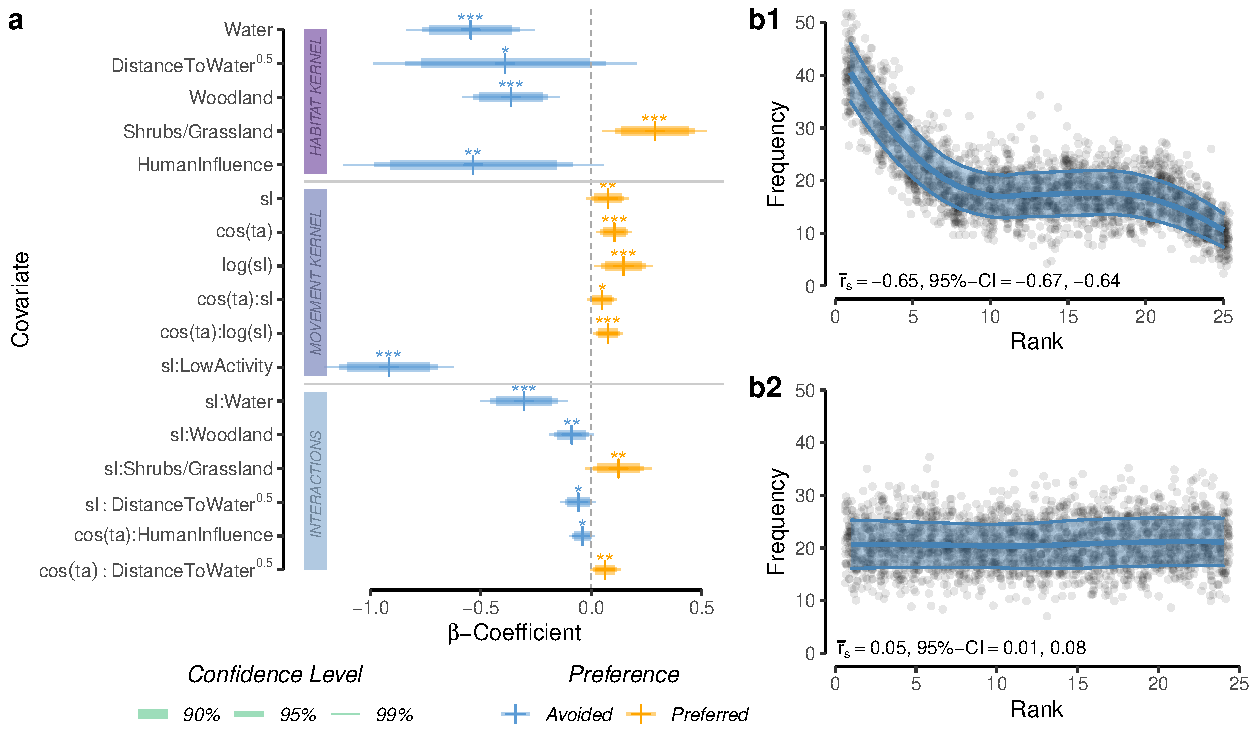
\includegraphics[width=\textwidth]{99_MovementModel}
    \caption{(a) Most parsimonious movement model for dispersing wild dogs. The
    model comprises a habitat kernel, a movement kernel, as well as their
    interactions. The horizontal line segments delineate the 90\%, 95\%, and
    99\% confidence-intervals for the respective \(\beta\)-coefficients.
    Significance codes: * \(p < 0.10\), ** \(p < 0.05\), *** \(p < 0.01\). (b)
    Results from the k-fold cross validation procedure. The upper plot shows
    rank frequencies of realized steps according to model predictions with known
    preferences, whereas the lower plot shows rank frequencies of realized steps
    when assuming random preferences. The blue ribbon shows the prediction
    interval around a loess smoothing regression that we fitted to ease the
    interpretation of the plots. The significant correlation between rank and
    associated frequency in (b1) highlights that the most parsimonious model
    successfully outperforms a random guess (b2) and assigns comparably high
    selection scores to realized steps.}
    \label{MovementModel}
  \end{center}
\end{figure}

\subsection{Dispersal Simulation}
Dispersal simulations based on the most parsimonious movement model proved
useful for assessing landscape connectivity. Of the 50,000 simulated dispersers
initiated within the main study area, only 4.5\% were eventually repelled by a
map boundary, suggesting minimal biases due to boundary effects. Moreover, our
examination of the relative traversal frequency across all checkpoints showed
that connectivity reached a steady state after 10,500 simulated dispersal
trajectories (Figure S3). Although variability in relative traversal frequency
kept decreasing as we increased the number of simulated dispersers, the marginal
benefit of additional trajectories diminished quickly (Figure S3).

\subsection{Heatmap}
The heatmap (\Cref{Heatmap}), which resulted from the summation of all simulated
dispersal trajectories, showed that several extensive regions within the
KAZA-TFCA were frequently traversed by dispersing wild dogs (mean traversal
frequency inside KAZA-TFCA = 166, IQR = 274, Figure S6a), whereas areas beyond
the KAZA-TFCA boundary were rarely visited (mean traversal frequency outside
KAZA-TFCA = 61, IQR = 133, Figure S6a). Most notably, the region in northern
Botswana south of the Linyanti swamp appeared as highly frequented dispersal
hotspot (mean traversal frequency = 987, IQR = 558). Nevertheless, the presence
of extensive water bodies, such as the Okavango Delta, the Makgadikgadi Pan, and
the Linyanti swamp, restricted dispersal movements and limited realized
connectivity within the KAZA-TFCA. Similarly, high human density, roads, and
agricultural activities in Zambia's and Zimbabwe's part of the KAZA-TFCA limited
dispersal movements in those countries. Outside the KAZA-TFCA, the most heavily
used regions included the areas inside the Central Kalahari National Park in
Botswana, the area south-west of the Khaudum National Park in Namibia, and the
area surrounding the Liuwa Plains National Park in Zambia. Although the heatmap
facilitated the identification of areas frequently traversed by simulated
dispersers, it seemed impractical to pinpoint dispersal corridors.

\begin{figure}
  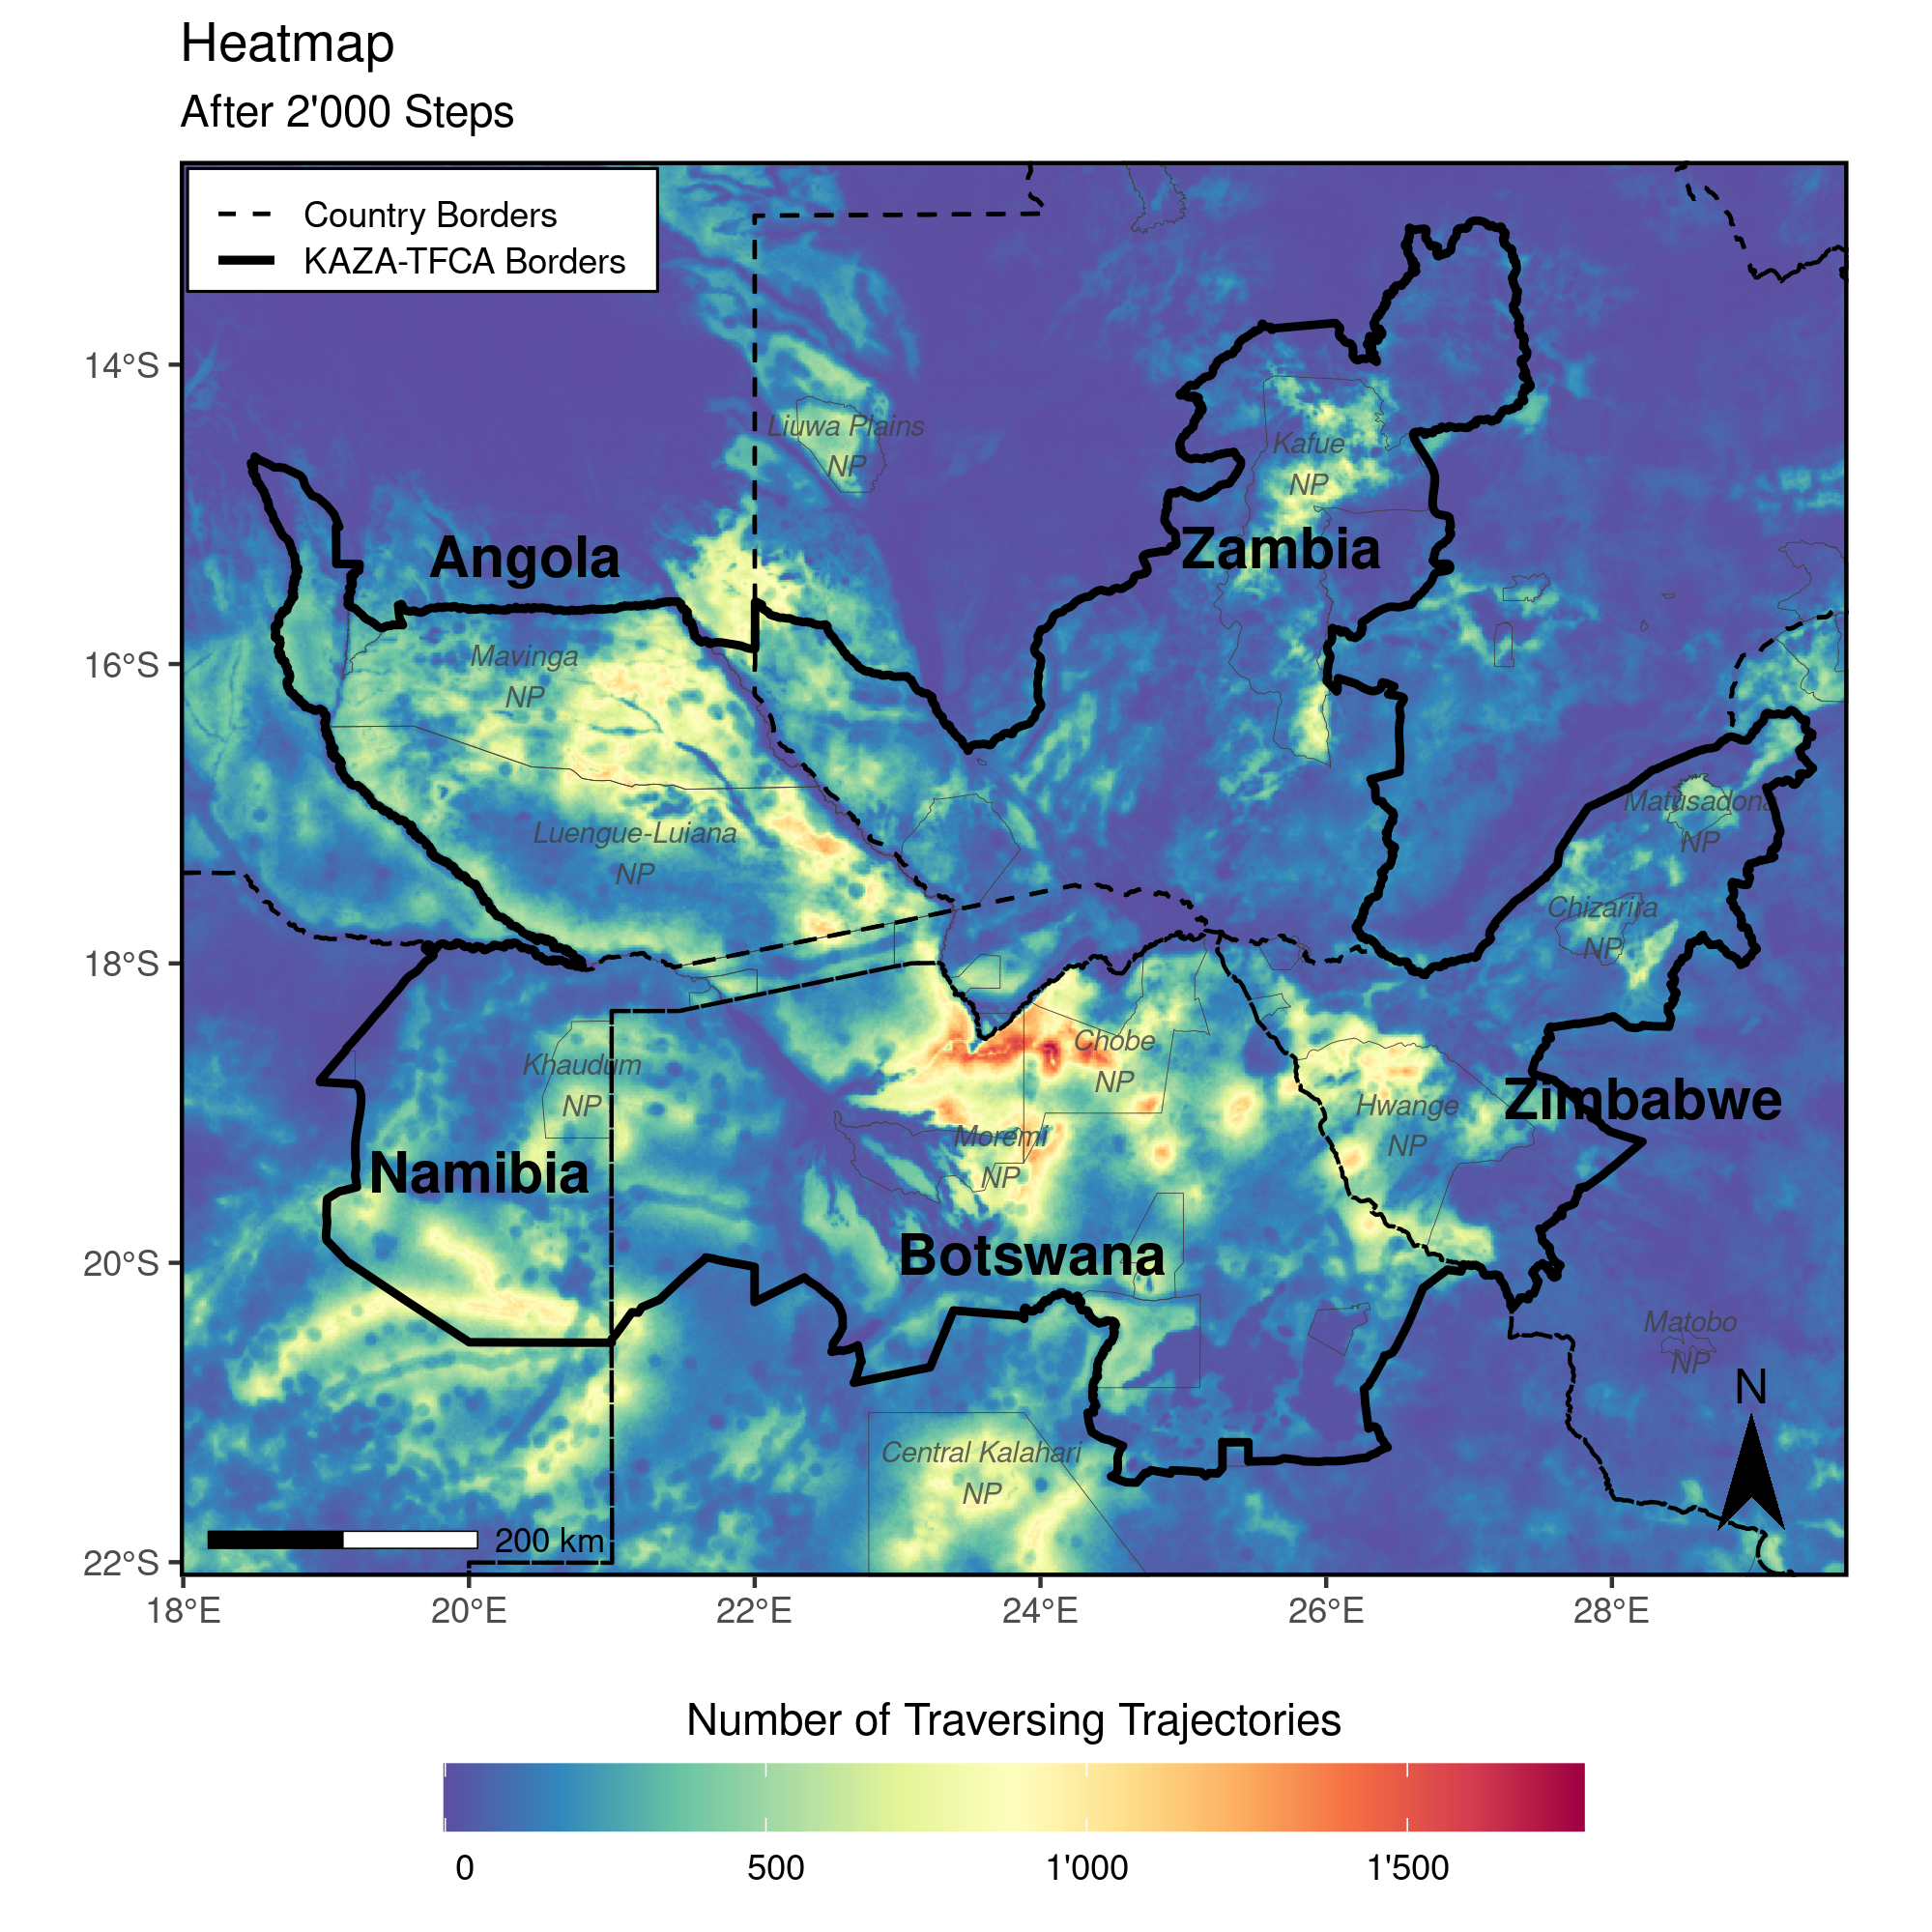
\includegraphics[width=\textwidth]{99_Heatmap.png}
  \caption{Heatmap showing traversal frequencies of 80'000 simulated dispersers
  moving 2'000 steps across the KAZA-TFCA. Simulations were based on an
  integrated step selection model that we fitted to the movement data of
  dispersing African wild dogs. To generate the heatmap, we rasterized and
  tallied all simulated trajectories. Consequently, the map highlights areas
  that are frequently traversed by virtual dispersers. For spatial reference we
  plotted a few selected NPs (dark gray). Additional heatmaps showing the
  traversal frequency when individuals move fewer than 2'000 steps are provided
  in Figure S4.}
  \label{Heatmap}
\end{figure}

\subsection{Betweenness}
The betweenness map (\Cref{Betweenness}) revealed distinct dispersal corridors
that run within the KAZA-TFCA. Again, the region in northern Botswana emerged as
a wild dog dispersal hub that connected more remote regions in the study area.
Towards east, the extension of this corridor ran through Chobe National Park
into Hwange National Park. From there, a further extension connected to
Matusadona National Park in Zimbabwe. Northwest of the Linyanty ecosystem, a
major corridor expanded into Angola, where it split and finally traversed
over a long stretch of unprotected area into Zambia's Kafue National Park.
Several additional corridors with lower betweenness scores emerged, yet most of
them ran within the KAZA-TFCA boundaries (median betweenness inside KAZA-TFCA =
6.947 Mio, IQR = 54.311 Mio, Figure S6b). In general, there were few corridors
that directly linked the peripheral regions of the KAZA-TFCA and passed through
unprotected areas outside the KAZA-TFCA (mean betweenness outside KAZA-TFCA =
2.685 Mio, IQR = 9.891 Mio, Figure S6b). Compared to the heatmap, the
betweenness map facilitated the identification of dispersal corridors between
habitat patches.

%  9 2000  Betweenness Inside KAZA-TFCA  6946817.   54311358.
% 10 2000  Betweenness Outside KAZA-TFCA 2685174.    9890504.

\begin{figure}
  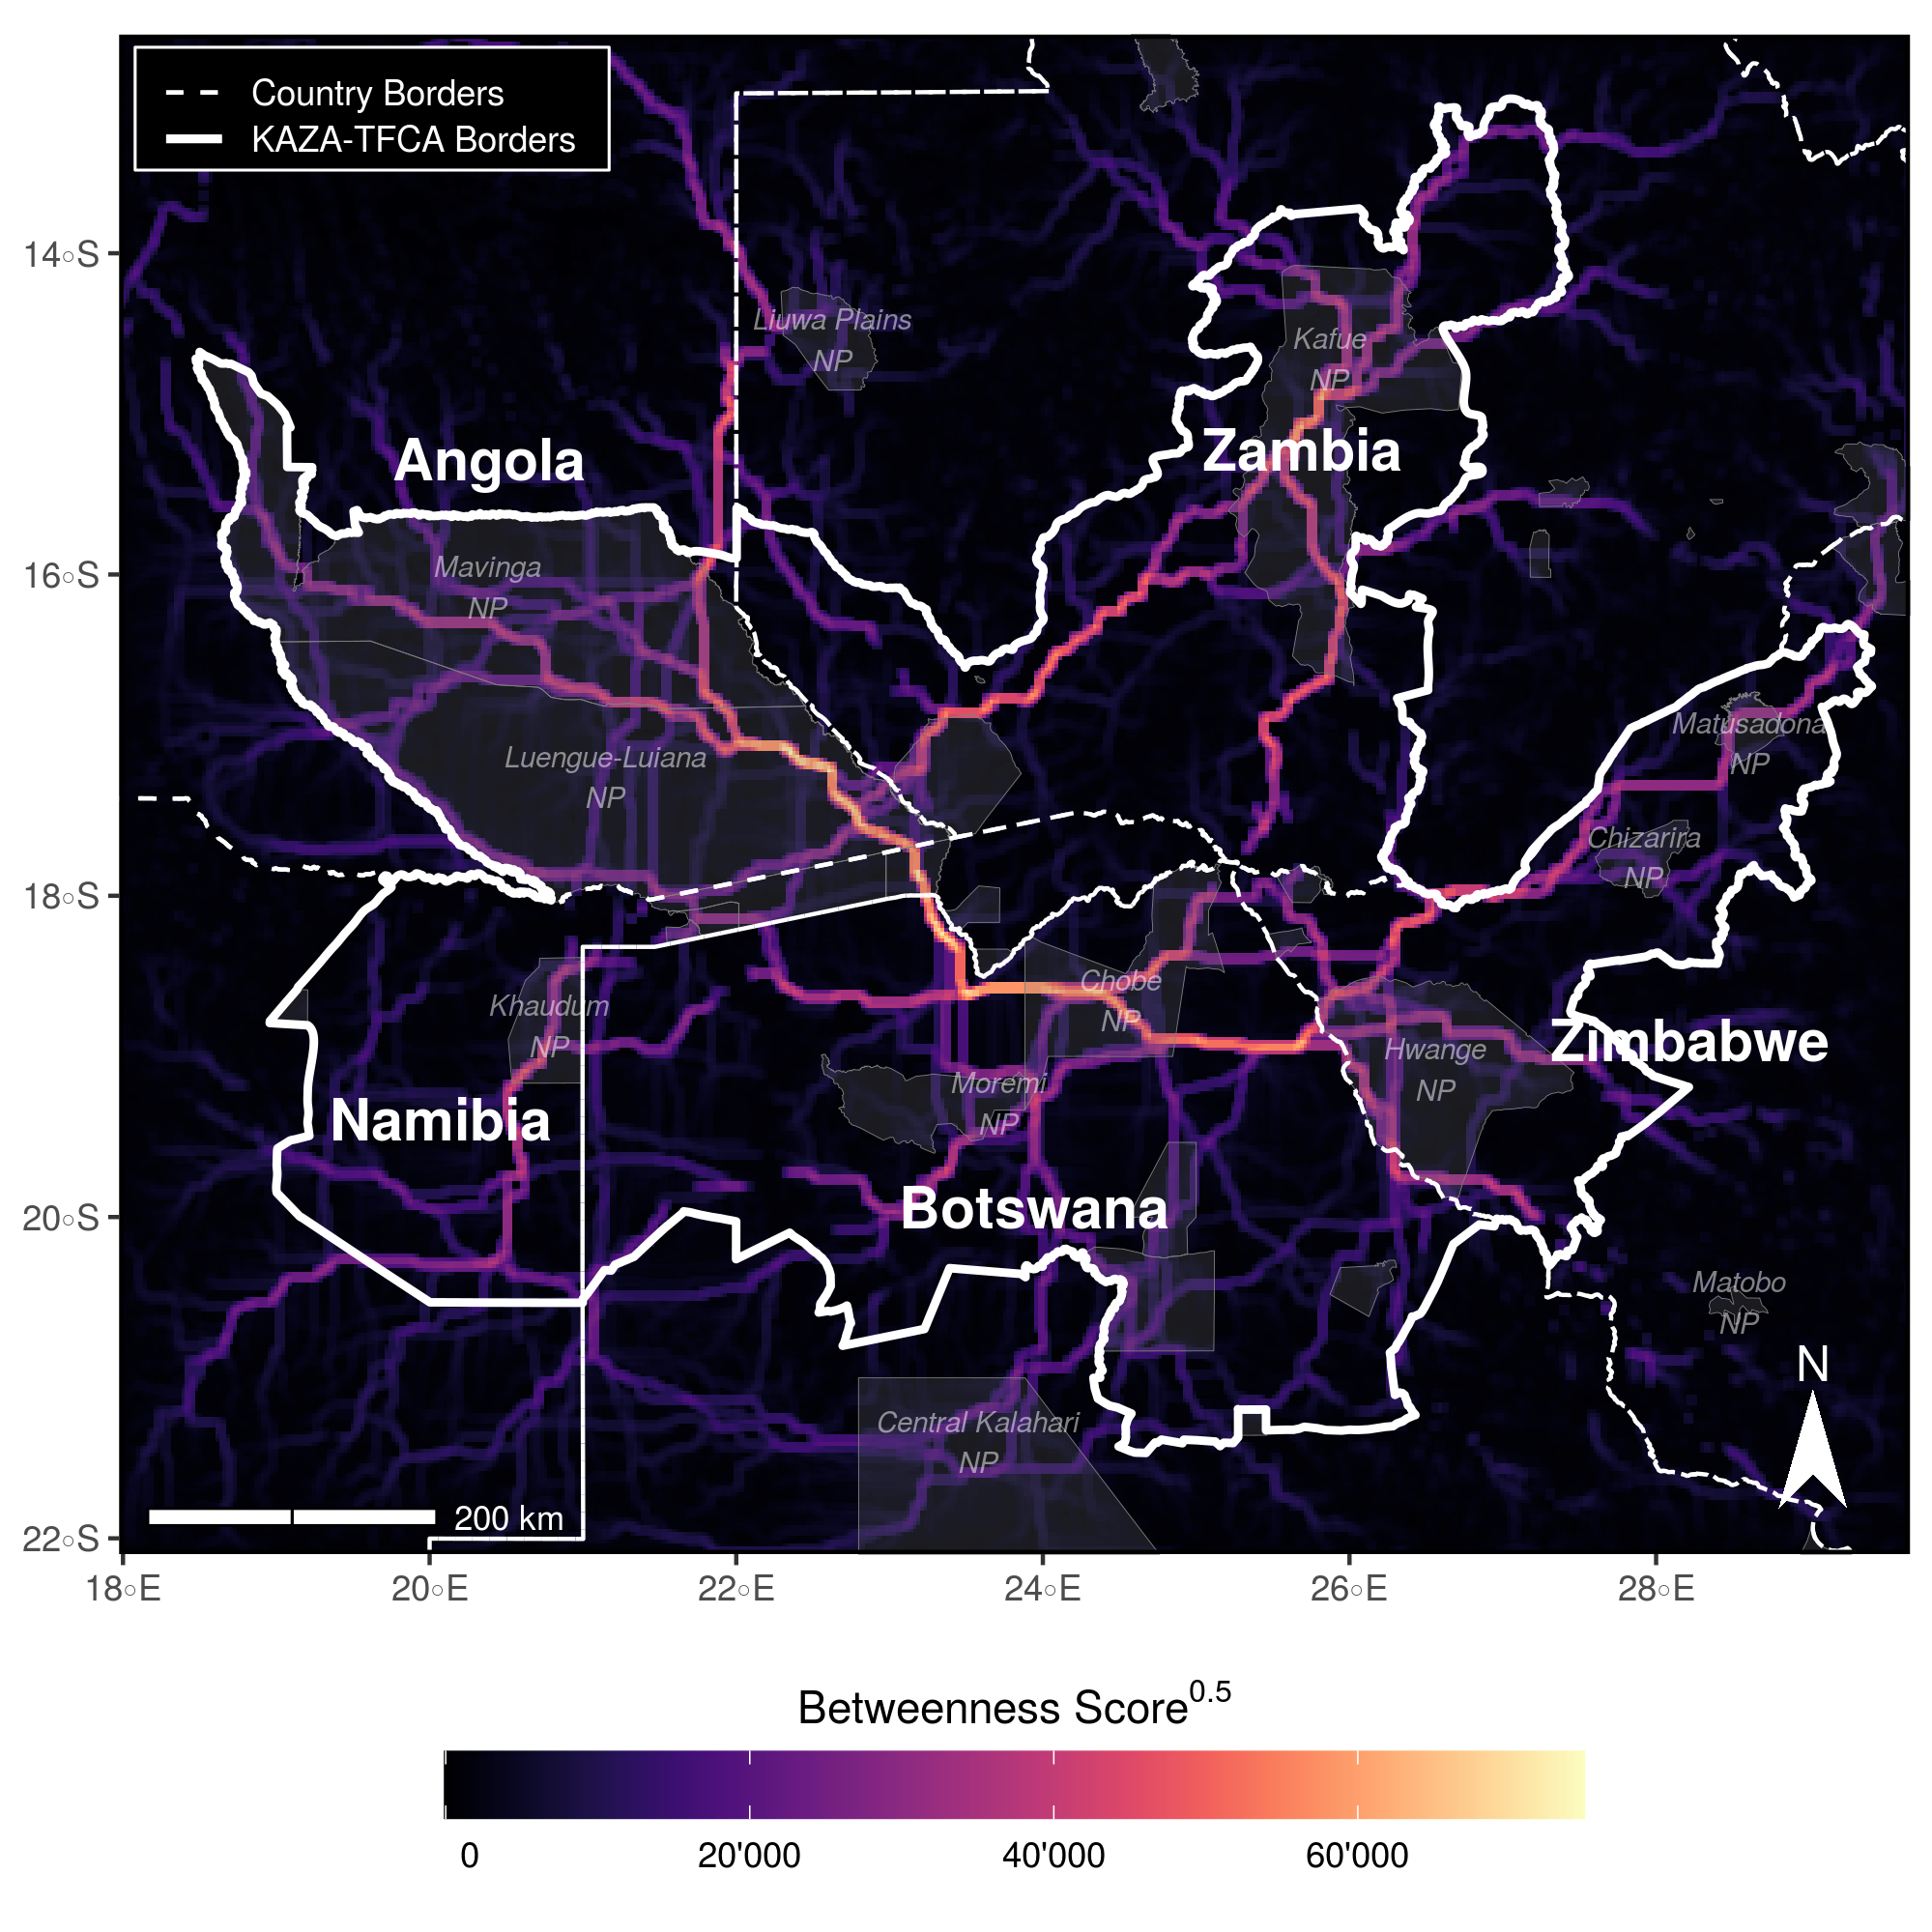
\includegraphics[width=\textwidth]{99_Betweenness.png}
  \caption{Map of betweenness scores, highlighting distinct dispersal corridors
  and potential bottlenecks across the extent of the KAZA-TFCA. Betweenness
  measures the number of shortest paths traversing through each node
  (raster-cell). Hence, a high betweenness score indicates that the respective
  area is exceptionally important for connecting different regions in the study
  area. The metric is therefore useful to pinpoint discrete movement corridors
  \citep{BastilleRousseau.2018}. Note that we square-rooted betweenness scores
  to improve visibility of corridors with comparably low scores. Additional
  betweenness maps showing betweenness scores when individuals move fewer than
  2'000 steps are provided in Figure S4.}
  \label{Betweenness}
\end{figure}

\subsection{Inter-Patch Connectivity}
The map of inter-patch connectivity showed that the relative frequency at which
simulated dispersers moved from one NP to another varied, as did the average
dispersal duration required to make these connections
(\Cref{InterpatchConnectivity}). Overall, inter-patch connectivity between NPs
in Angola, Namibia, Botswana, and Zimbabwe appeared to be high; between 54\% and
87\% of individuals originating from a NP in these countries successfully moved
into some other NP (Figure S6a). Conversely, only 19\% of the dispersers leaving
from a NP in Zambia managed to find a route into some other NP (Figure S6b).
Prior to reaching another NP, individuals from Angola, Namibia, Botswana,
Zimbabwe, and Zambia had to move for an average of 630, 640, 940, 1045, and 890
steps, respectively. For some NPs, we also detected imbalances between the
number of ingoing and outgoing links, hinting at possible source-sink dynamics.
From Chobe NP, for instance, 510 individuals reached Moremi NP, yet the opposite
route was only realized by 340 individuals. However, relative to the number of
simulated individuals in these NPs, these numbers imply fractions of 50\% and
68\%. Interestingly, it also appears that the dispersal corridor between
Angola's NPs and the Kafue NP in Zambia identified in
\Cref{InterpatchConnectivity} is only rarely realized.

\begin{figure}
  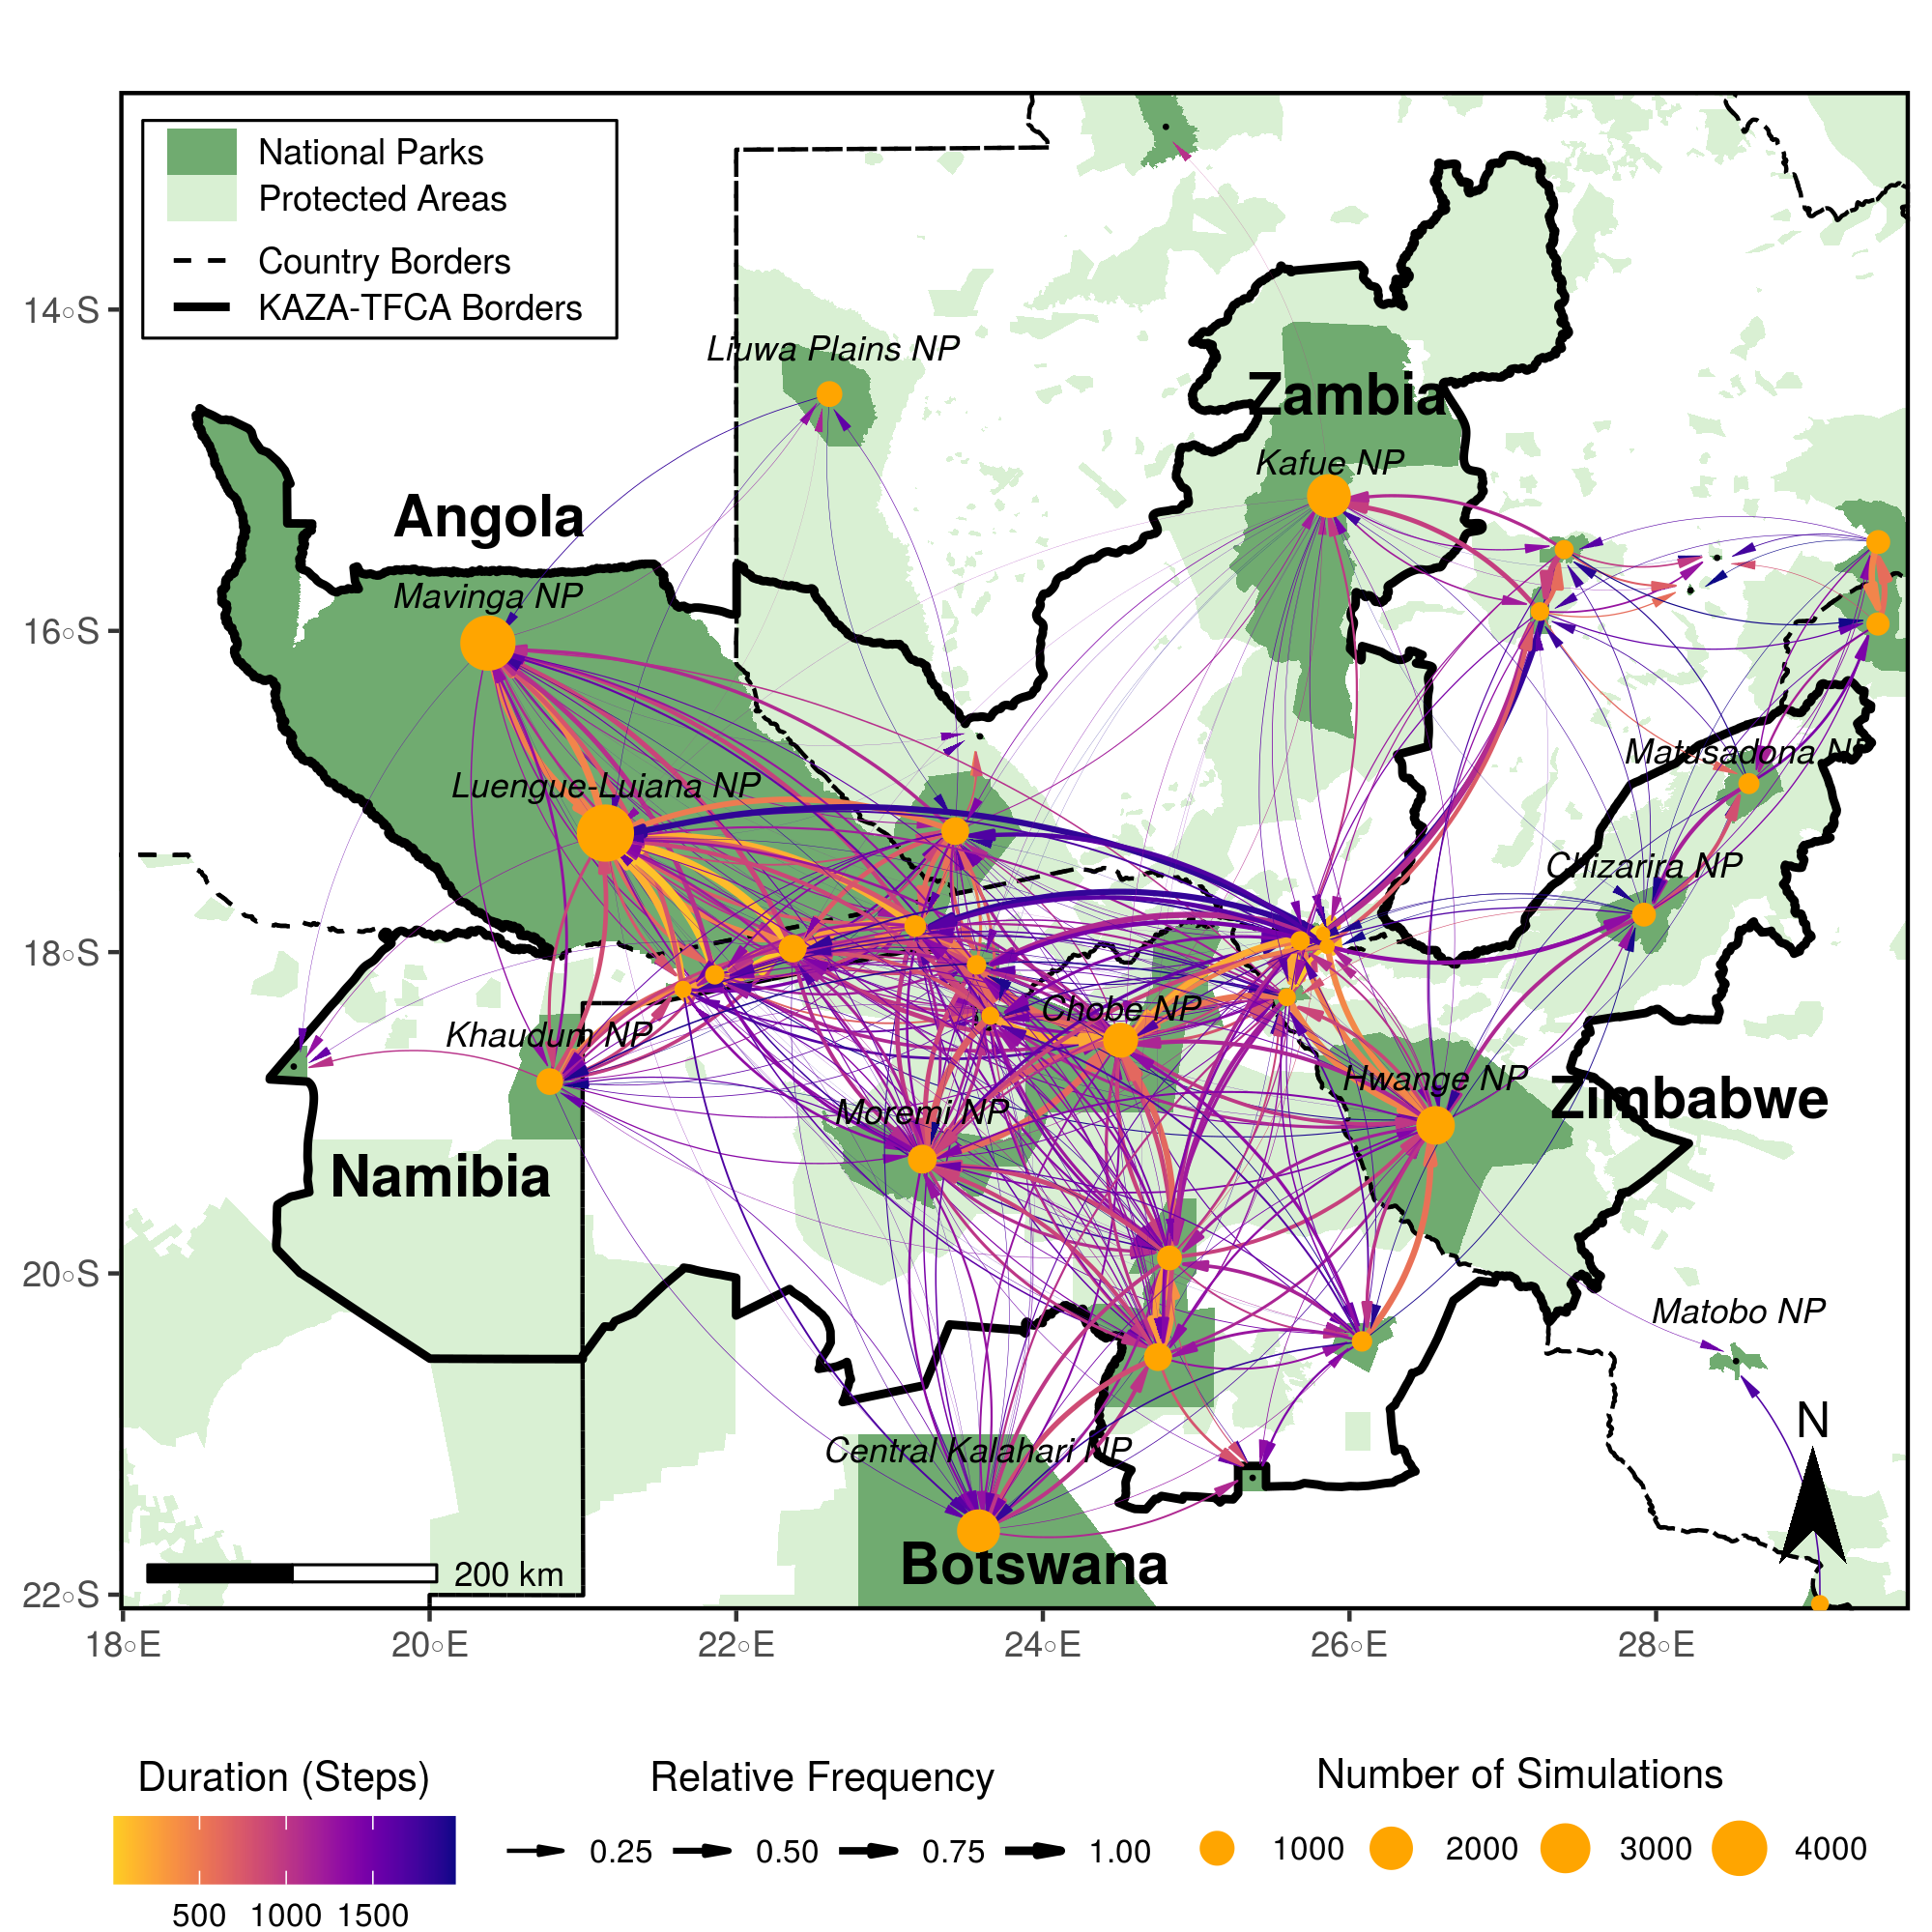
\includegraphics[width=\textwidth]{99_InterpatchConnectivity.png}
  \caption{Map of inter-patch connectivity, highlighting connections between NPs
  (dark green). Yellow bubbles represent the center of the different NPs and are
  sized in relation to the number of simulated dispersers originating from each
  park. Black dots represent NPs that were smaller than 700
  km\textsuperscript{2} and therefore did not serve as source areas. Arrows
  between NPs illustrate between which NPs the simulated dispersers successfully
  moved and the color of each arrow shows the average number of steps (4-hourly
  movements) that were necessary to realize those connections. Additionally, the
  line thickness indicates the relative number of dispersers originating from a
  NP that realized those connections. Note that a similar network view could be
  adopted to investigate connectivity between other protected areas need not to
  be restricted to NPs.}
  \label{InterpatchConnectivity}
\end{figure}

\section{Discussion}

% Short Summary
\subsection{Short Summary}
We presented a three-step workflow to simulate dispersal and assess landscape
connectivity. We also demonstrated application of the three steps using
empirical dispersal data from a free-ranging population of African wild dogs. In
step one, we used ISSFs to parametrize a fully mechanistic movement model
describing how dispersing wild dogs move through the available landscape. In
step two, we employed the fitted model to simulate 80,000 dispersing wild dogs
moving 2,000 steps across the extent of the KAZA-TFCA, the world's largest
transboundary conservation area. In step three, we converted simulations into
three complementary connectivity maps, each emphasizing a different aspect of
landscape connectivity. The set of maps included a heatmap revealing frequently
traversed areas, a betweenness-map delineating critical dispersal corridors, and
a map of inter-patch connectivity indicating the presence and intensity of
functional links between NPs and the average dispersal duration required to make
those links. With this, we showed that simulations from ISSFs overcome several
conceptual shortcomings inherent to more traditional connectivity modeling
techniques, such as LCPA and CT.

% Movement Model
\subsection{Movement Model}
Our movement model of dispersing wild dogs, which included interactions between
habitat and movement covariates, effectively rendered habitat and movement
preferences of dispersers, leading to a significant improvement in predictive
performance compared to an earlier model that omitted such interactions
\citep{Hofmann.2021}. Results on habitat preferences largely complied with
previous studies that investigated habitat selection by dispersing wild dogs
\citep{DaviesMostert.2012, Masenga.2016, Woodroffe.2019, Oneill.2020,
Hofmann.2021}, yet by also rendering movement preferences, we were able to model
several additional complexities common to dispersal. For instance, by including
the appropriate interactions in the movement model we could accommodate that
dispersers move with directional persistence and exhibit step lengths that are
correlated with turning angles. Albeit the same autocorrelation could be
rendered by sampling step lengths and turning angles from copula probability
distributions \citep{Hodel.2021a, Hodel.2021b}, the ISSF framework allowed us to
incorporate correlations directly in the movement model. We only considered
first order autocorrelation, i.e. correlation between two consecutive steps,
although higher order autocorrelation is conceivable and may be desirable to
model \citep{Dray.2010, McClintock.2012}. This will require vast amounts of GPS
data that are not interrupted by missing fixes; something that is rarely
achieved in reality \citep{Graves.2006}. Aside from modeling autocorrelation in
consecutive movements, we also rendered potential dependencies between movement
and habitat preferences by forming interactions between habitat covariates and
movement covariates. For example, our final model contained an interaction
between water-cover and step lengths showing that dispersers realized shorter
steps in areas covered by water or an interaction between turning angles and
water-cover highlighting that dispersers moved more tortuous in areas covered by
water. The results themselves are not surprising, considering that wild dogs can
only cross water by swimming or wading. Nevertheless, the ability of
accompanying such effects in a single model is what makes ISSFs such a great and
flexible tool for rendering a variety of different movement behaviors
\citep{Avgar.2016, Fieberg.2021}. For this reason, we believe the method is a
perfectly suited framework for individual-based simulations that serve to
examine connectivity.

\subsection{Simulation}
Our simulation of 80'000 dispersers moving 2'000 steps across the KAZA-TFCA
required five days of computation on a modern desktop machine (AMD Ryzen 7 2700X
processor with 8 x 3.6 GHz and 16 logical cores, 64 GB of RAM). The long
simulation time was primarily caused by the massive extent considered (ca. 1.8
Mio km\textsuperscript{2}) and the large number of dispersers simulated. Most
connectivity studies are limited to smaller extents (e.g.
\citealp{Kanagaraj.2013, Clark.2015, McClure.2016, Abrahms.2017, Zeller.2020})
and will therefore achieve faster simulation times. We also believe that fewer
simulated dispersers will often suffice, as the relative traversal frequency by
simulated individuals through randomly placed checkpoints across our study area
converged already after 10,500 simulated dispersal trajectories. The number of
required simulations to achieve reliable estimates of connectivity will,
however, vary depending on the structure of the landscape and the dispersal
ability of the focal species \citep{Gustafson.1996}. For species that disperse
short distances through homogeneous environments, already few simulations may
suffice go gauge connectivity, whereas for species that disperse over long
distances through heterogeneous habitats, a large number of simulations will be
required to sufficiently explore the spectrum of possible routes.

\subsection{Maps}
Each of the three connectivity maps derived from simulated dispersal
trajectories highlighted a different aspect of landscape connectivity. The
heatmap was most suitable for pinpointing frequently traversed areas and showed
that an exceptionally large number of dispersers moved through the regions of
the Moremi NP and the Chobe NP in northern Botswana. We previously identified
the same area as potential dispersal hotspot using LCPA \citep{Hofmann.2021},
yet it was not clear whether this was a consequence of the region being located
in the center of the study area and connections being enforced between
predefined start and endpoints. Contrary to LCPA, a simulation-based approach as
presented in this paper does not require predefined endpoints because endpoints
emerge naturally as the result from a simulated dispersal trajectories. Not
having to pre-determine endpoints is especially useful for dispersal studies, as
known endpoints are usually an unrealistic assumption \citep{Elliot.2014,
Abrahms.2017, Cozzi.2020}. Simultaneously, simulations permit to detect
potential routes that do not necessarily lead into suitable habitats but into
ecological traps \citep{Dwernychuk.1972, VanDerMeer.2014} or into areas with a
high susceptibility for human wildlife conflicts \citep{Cushman.2018}.
Irrespective of the fact that simulated individuals were no longer enforced to
move towards known endpoints, numerous simulated individuals traversed
the region in northern Botswana, demonstrating that this hotspot is not merely
an artifact but truly results from its favorable landscape characteristics.

In contrast to the heatmap, the betweenness map emphasized relatively narrow and
linear movement routes and thus facilitated the identification of discrete
movement corridors in the study area. The resulting map reinforced our notion
that Botswana plays a central role for the establishment of connections into
more remote regions of the KAZA-TFCA. While in this case both the heatmap and
the betweenness map attribute high importance to the region in northern
Botswana, there are other regions in which the two metrics do not necessarily
coincide. The stretch of unprotected land between Luengue-Luiana NP in Angola
and the Kafue NP in Zambia, for instance, receives a high betweenness-score, yet
is only rarely traversed by dispersers according to the heatmap. This implies
that the corridor takes on a crucial role for connecting Luengue-Luiana NP to
Kafue NP, yet is in reality only traversed rarely. These contrasts highlight the
value of consulting multiple metrics when assessing connectivity.

As a final piece to the trinity of connectivity maps, we produced a map of
inter-patch connectivity that strictly focused on NPs. The map depicted the
frequency at which simulated individuals moved between NPs as well as the
average duration (in steps) required to realize them. Calculating dispersal
durations was only possible because dispersal trajectories were simulated
spatio-temporally explicitly, something that is currently impossible using LCPA
or CT. An explicit representation of time enables to answer questions such as:
``\textit{How long will it take a disperser to move from A to B?}'' or
``\textit{Is it possible for a disperser to move from A to B within X days?}''.
Moreover, rendering time explicitly yields opportunities to study how
seasonality affects connectivity and to investigate whether dispersal corridors
are only available temporarily or all-year round (\textit{dynamic connectivity};
\citealp{Zeller.2020}). With LCPA or CT, seasonality can currently only be
incorporated by generating seasonal permeability surfaces and repeating the
connectivity analysis for each surface individually (e.g. \citealp{Benz.2016,
Osipova.2019}). With simulations from ISSFs, on the other hand, seasonal changes
in the environment could be rendered dynamically ``as the dispersers move'', so
that simulated individuals could directly respond to such fluctuations.

\subsection{Disadvantages of ISSF Simulations}
Despite the many benefits and great flexibility offered by simulations from
ISSFs, one also must be aware of the associated non-trivial but important
modeling decisions. Here, we will elaborate on four modeling decisions
concerning: (1) the number of simulated individuals, (2) the location of source
points, (3) the simulated dispersal duration, and (4) behavior at map
boundaries.

(1) When simulating dispersal, the modeler needs to decide on the number of
simulated individuals. A higher number is always desirable, as each additional
disperser provides information about landscape connectivity, yet every
individual also entails computational costs. Consequently, a trade-off needs to
be managed and the benefits of simulating additional dispersers needs to be
gauged against the cost of computation. \cite{Signer.2017} suggests handling
this trade-off by simulating additional individuals only until the metrics of
interest converge towards their steady state. We incorporated this idea and
employed the relative traversal frequency across randomly placed checkpoints to
verify that the number of simulated individuals was large enough. However, the
exact number of required individuals might vary depending on the target metric
and the anticipated connectivity map. More sophisticated target metrics tailored
for each connectivity map will need to be developed in the future.

(2) To initiate dispersers, a modeler needs to provide a set of source points.
We placed source points within protected areas large enough to sustain viable
wild dog populations, implicitly assuming wild dogs would primarily survive in
large, formally protected areas \citep{Woodroffe.1999, DaviesMostert.2012,
Woodroffe.2012, VanDerMeer.2014}. We lacked precise knowledge about wild dog
densities in the different protected areas, so we distributed source points
within them randomly. In cases where such data is available (e.g. thanks to a
habitat suitability model; \citealp{Squires.2013}), source points can be
distributed accordingly, reflecting that the number of dispersers may not
strictly scale with the size of the source area. Alternatively, source points
can be distributed homogeneously across suitable habitats and only later be
weighted when deriving connectivity metrics. After all, the challenge of
selecting meaningful source points is not unique to individual-based simulations
but also applies to LCPA or CT.

(3) When employing ISSFs to simulate dispersers, it is required to decide on the
number of simulated steps (i.e. dispersal durations). If sufficient dispersal
data of the focal species has been collected, dispersal durations could be
sampled from observed dispersal events. In our case, the low number of observed
dispersal events and the high variability in wild dog dispersal durations (see
\citep{DaviesMostert.2012, Masenga.2016, Cozzi.2020, Hofmann.2021}) prevented us
from sampling from observed dispersal events. Instead, we simulated all
individuals for 2'000 steps, which is at the upper end of observed dispersal
durations. This allowed us to subsample trajectories to shorter durations after
their simulations and to investigate the sensitivity of our connectivity maps
with respect to exact dispersal durations (Figures S4 and S5).

(4) Unless simulated individuals are strongly drawn towards a point of
attraction (e.g. \cite{Signer.2017}), some individuals will inevitably approach
a map boundary such that one of their proposed random steps leaves the study
area. In theoretical applications, this problem can be circumvented by
simulating movement on a torus where no map boundaries exist \citep{Hodel.2022}.
For real world data, however, other approaches are needed. One possible solution
would be to simply terminate the simulation of the respective individual as soon
as one of its random steps transgresses a map border. This approach implicitly
assumes that the respective animal left the study area and will never return. In
cases where individuals are released near map borders, this approach will be
problematic, as already a single transgressing random step will break the
simulation, thus strongly biasing dispersal from patches near map borders. We
tried to mitigate this issue in two complementary ways. First, we artificially
increased covariate layers (and therefore the study area) by a buffer zone with
randomized covariate values. The same method has already proven effective in
mitigating edge-effects for graph-based methods \citep{Koen.2010}. In our case,
the buffer enabled dispersers to leave and re-enter the main study area, as well
as to initiate potential immigrants into our study system. As a second
mitigation measure, we resampled any transgressing random steps until they fully
lied within the study area, thus enforcing individuals to always remain within
the study area. Given that only very few simulated individuals were repelled by
a virtual map boundary, we conclude that the two measures effectively obviated
boundary effects.

\subsection{Conclusion}
To this end, we proposed and applied a simple three-step workflow that relies on
ISSF-analysis and enables to simulate dispersal and assess landscape
connectivity. The proposed workflow overcomes several of the conceptual
shortcomings inherent to LCPA and CT, such as the assumption of known endpoints,
and provides a highly flexible tool for investigating connectivity. In our case
study, the workflow proved useful to investigate landscape connectivity for the
endangered African wild dog within the KAZA-TFCA ecosystem and allowed us to
pinpoint frequently used corridors and dispersal hubs. We hope to have sparked
interest in the powerful framework of ISSFs for investigating dispersal
connectivity, while at the same time conferring some of the non-trivial modeling
decisions involved.

\section{Authors' Contributions}
D.D.H., D.M.B., A.O. and G.C. conceived the study and designed methodology;
D.M.B., G.C., and J.W.M. collected the data; D.D.H. and D.M.B. analysed the
data; G.C. and A.O. assisted with modeling; D.D.H., D.M.B., and G.C. wrote the
first draft of the manuscript and all authors contributed to the drafts at
several stages and gave final approval for publication.

\section{Data Availability}
GPS movement data of dispersing wild dogs is available on dryad
\citep{Hofmann.2021b}. Access to R-scripts that exemplify the application of the
proposed workflow using simulated data are provided through Github
(\url{https://github.com/DavidDHofmann/DispersalSimulation}). In addition, all
codes required for the African wild dog case study will be made available
through an online repository at the time of publication.

\section{Acknowledgements}
We thank the Ministry of Environment and Tourism of Botswana for granting
permission to conduct this research. We thank C. Botes, I. Clavadetscher, and G.
Camenisch for assisting with wild dog immobilizations. We also thank B. Abrahms
for sharing her data of three dispersing wild dogs. Furthermore, we would like
to thank Johannes Signer for assisting with the simulation algorithm. This study
was funded by Basler Stiftung für Biologische Forschung, Claraz Foundation, Idea
Wild, Jacot Foundation, National Geographic Society, Parrotia Stiftung, Stiftung
Temperatio, Wilderness Wildlife Trust Foundation, Forschungkredit der
Universität Zürich, and a Swiss National Science Foundation Grant
(31003A\_182286) to A. Ozgul.

\newpage
\begingroup
\singlespacing
\bibliography{Literatur}
\endgroup

\end{document}
